\section{Модальный регулятор}

Рассматриваем систему
\begin{equation}
    \dot x = Ax+Bu,\quad
    A=\begin{bmatrix}
        3 & 5 & 4 \\
        -2 & -4 & -5 \\
        2 & 2 & 3
    \end{bmatrix},\quad
    B=\begin{bmatrix}
        2 \\ -1 \\ 1
    \end{bmatrix}.
    \label{eq:1}
\end{equation}
Спектр матрицы $A$
\begin{equation*}
    \sigma(A)=\{2\pm i,\ -2\}.
\end{equation*}
Построив матрицы Хаутуса, сделаем вывод, что сопряженная пара
собственных чисел управляема, а вещественное число $-2$ - нет,
но так как оно отрицательное, то система стабилизируема, хотя и
не полностю управляема. 

Построим структурную схему системы Рис. \ref{fig:1}.
\begin{figure}[H]
    \centering
    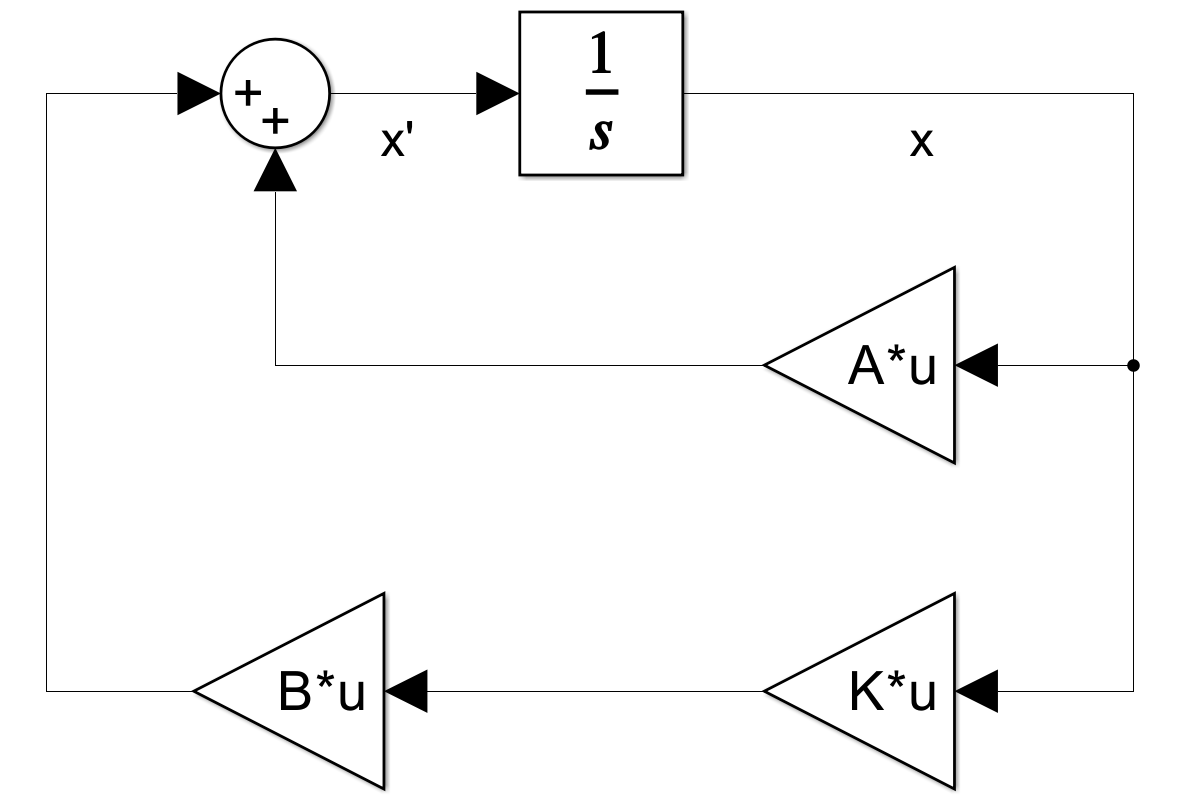
\includegraphics[width=0.7\linewidth]{figs/task1_slx.png}
    \caption{Схема моделирования системы \ref{eq:1}, замкнутой
    регулятором вида $u=Kx$}
    \label{fig:1}
\end{figure}
Предложены данные варианты спектра $\sigma(A+BK)$
\begin{equation*}
    \begin{array}{rl}
        \{-1,\ -1,\ -1\}, & \{-2,\ -2,\ -2\}, \\
        \{-1,\ -10,\ -100\}, & \{-2,\ -20,\ -200\}, \\
        \{-1,\ -1\pm 3i\}, & \{-2,\ -2\pm 6i\}.
    \end{array}
\end{equation*}
Спектры, которые не содержат $-2$ недостежимы, так как
данное собственное число неуправляемо, оно всегда будет
присутствовать в спектре системы. Оставшиеся
3 спектра достежимы.